\documentclass{article}

% Language setting
% Replace `english' with e.g. `spanish' to change the document language
\usepackage{cmap}					% поиск в PDF
\usepackage[T2A]{fontenc}			% кодировка
\usepackage[utf8]{inputenc}			% кодировка исходного текста
\usepackage[english,russian]{babel}	 

% Set page size and margins
% Replace `letterpaper' with `a4paper' for UK/EU standard size
\usepackage[letterpaper,top=2cm,bottom=2cm,left=3cm,right=3cm,marginparwidth=1.75cm]{geometry}

% Useful packages
\usepackage{amsmath}
\usepackage{graphicx}
\usepackage[colorlinks=true, allcolors=blue]{hyperref}

\title{Решение системы линейных уравнений методом наискорейшего градиентного спуска}
\author{ИВТ-22}

\begin{document}
\maketitle

\section{Описание метода}

  
Метод наискорейшего градиентного спуска является итерационным методом решения систем линейных уравнений.
Метод применяется для решения систем вида 

\begin{equation}
    Ax = b,
\end{equation}
где $A$ --- положительно определенная симметричная матрица коэффициентов, $b$ --- вектор правых частей 
системы, $x$ --- вектор неизвестных.  


Метод заключается в построении последовательности векторов ${x_k}, \ k = 0, 1, 2, \dots$, сходящейся к
вектору $\xi$ --- решению системы (1). Рассмотрим функцию 

\begin{equation}
    f(x) = (Ax, x) - 2 (x, b)
\end{equation}  

Данная функция является квадратичной относительно координат вектора $x$, так как содержит 
члены второго порядка по этим координатам:
\begin{equation*}
    f(x) = \sum_{i} \sum_j a_{ij} x_i x_j - 2 \sum_i x_i b_i
\end{equation*}  


Покажем, что точка минимума функции $f(x)$ существует и является решением $\xi$ системы уравнений (1).  


Так как матрица системы (1) положительно определена, то определитель матрицы системы не равен нулю. Следовательно, система имеет единственное решение. Пусть $x$ = $\xi$ + $\Delta$ --- произвольный вектор,
тогда значение функции в $x$ равно:
\begin{align*}
    f(x) = f(\xi + \Delta) &= (A(\xi + \Delta), \xi + \Delta) - 2(\xi + \Delta, b) \\
    &= (A \xi, \xi) + (A \xi, \Delta) + (A \Delta, \xi) + (A \Delta, \Delta) - 
    2((\xi, b) + (\Delta, b)) \\
    &= f(\xi) + (A \xi - b, \Delta) + (A \Delta, \Delta) \geq f(\xi)
\end{align*}

Таким образом, $f(x)$ ограничена снизу значением $f(\xi)$. 

Введем понятие невязки, показывающее, насколько на $i$-м шаге $Ax_i$ отличается от $b$, то есть

\begin{equation}
    r_i =  b - Ax_i
\end{equation}

Найдем градиент $\nabla f$ функции $f(x)$. Пусть $p$ --- произвольный единичный вектор. Тогда, 

\begin{equation*}
    f(x + tp) = f(x) + 2tf(Ax - b, p) + t^2 (Ap, p).
\end{equation*}

Найдем значение, при котором производная достигает максимума, то есть найдем производную функции одной переменной
$f(t)$, при условии, что $t = 0$:

\begin{equation}
    \frac{df(x + tp)}{dt} \Bigr|_{t=0} = 2(Ax - b, p) = 2 |Ax - b| \cos \varphi,
\end{equation}

где $\varphi$ --- угол между $Ax - b$ и $p$, и заметим, что при $\varphi = 0$ производная достигает максимального значения, 
то есть, когда векторы $p$ и $Ax - b$ сонаправлены. Таким образом, градиент функции:

\begin{equation*}
    \nabla f = Ax - b = -r.
\end{equation*}

Введем итерационный процесс:

\begin{equation}
    x_{i + 1} = x_{i} + \alpha_{i} \cdot p_{i} = x_{i} + \alpha_i \nabla f= x_i + \alpha_i r_i
\end{equation}

Функция $f(x)$ убывает при движении в направлении вектора $r_i$ от точки $x_i$ до
тех пор, пока луч $x_i + t\cdot r_i, \ t > 0$, не достигнет более низкого множества
уровня функции $f(x)$. В такой точке касания $x_{i + 1}$ функция $f(x)$ достигает минимального значения локально, 
при этом $f(x_i + 1) < f(x_i)$.

\begin{figure}[h]
    \centering
    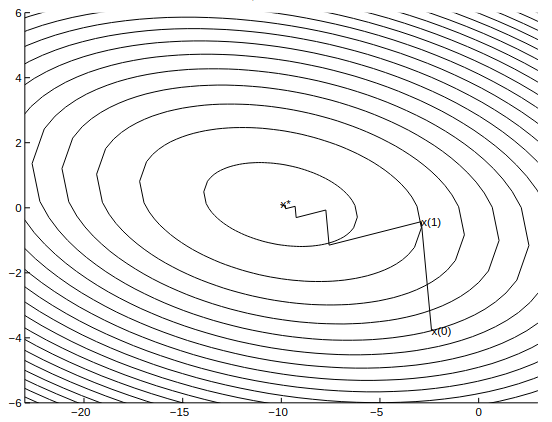
\includegraphics[width=0.5\linewidth]{image.png}
\end{figure}

Для определения коэффициента шага в (5) найдем минимум функции $f(x_i + \alpha_i r_i)$:

\begin{equation*}
    \frac{df(x_i + \alpha_i r_i)}{d\alpha_i} = 0
\end{equation*}

\begin{equation*}
    d(f(x_i) + 2\alpha_i (A x_i, r_i) + t^2 (A r_i, r_i) - 2 \alpha_i (b, r_i)) = 0
\end{equation*}

\begin{equation*}
    2(A x_i - b, r_i) + 2 \alpha_i (A r_i, r_i) = 0    
\end{equation*}

\begin{equation*}
    \alpha_i = \frac{(r_i, r_i)}{(A r_i, r_i)}
\end{equation*}

Если матрица не симметрична, то части равенства $Ax = b$ можно домножить на транспонированную матрицу $A^T$:

\begin{equation*}
    A^T A x = A^T b,
\end{equation*}

получив равносильную систему, матрица которой симметрична и положительно определена.

\section{Алгоритм}

Объединив полученные формулы, имеем:

\begin{equation}
    r_i = b - Ax_i
\end{equation}

\begin{equation}
    \alpha_i = \frac{(r_i, r_i)}{(A r_i, r_i)}
\end{equation}

\begin{equation}
    x_{i + 1} = x_i + \alpha_i \cdot r_i
\end{equation}

Данный рекуррентный алгоритм требует два произведения матрица-вектор за итерацию. Вычислительная сложность алгоритма, зависящая от этой 
операции, может быть упрощена, если в уравнении (8) умножить обе части равенства на $-A$ и прибавить $b$:

\begin{equation}
    r_{i + 1} = r_i - \alpha_i A r_i.
\end{equation}

Произведение $Ar$, которое используется в уравнениях (7) и (9), можно вычислить только один раз. Недостатком 
такой оптимизации является то, что в уравнении (9) не используется значение $x_i$, то есть отсутствует обратная связь по $x$.
Таким образом накопление ошибки округления может привести к сходимости последовательности ${x_i}$ к точке, не совпадающей с
решением системы уравнений. Этого можно избежать, если раз в определенное число итераций пересчитывать $Ax$.

 
\begin{thebibliography}{9}

\bibitem{1}
  \url{https://books-vuzi.narod.ru/olderfiles/1/VICH_MATH_MAXIMA.PDF}



\bibitem{2}
  \url{https://users.cs.utah.edu/~haocheng/notes/NoteonConjugateGradientMethod.pdf}

\bibitem{3}
  \url{https://antonleykin.math.gatech.edu/math2605fall10/PROJECTS/SteepestDescent.pdf}


\bibitem{4}
  \url{https://ocw.mit.edu/courses/18-409-topics-in-theoretical-computer-science-an-algorithmists-toolkit-fall-2009/68f1b1ba4d419ee8f3b67a41ebf258e8_MIT18_409F09_scribe21.pdf}


\bibitem{5}
  \url{https://antonleykin.math.gatech.edu/math2605fall10/PROJECTS/SteepestDescent.pdf}

\bibitem{5}
  \url{https://www.cs.umd.edu/users/oleary/a600/cgnotes.pdf}


\bibitem{5}
  \url{https://people.eecs.berkeley.edu/~satishr/cs270/sp11/rough-notes/Linear-Equations.pdf}


\bibitem{5}
  \url{https://www.phys.uconn.edu/~rozman/Courses/m3511_18s/downloads/steepest-descent.pdf}

\end{thebibliography}

\end{document}
